\newcommand{\figureSPIShiftRegister}[1]{
  \def\lang{\detokenize{#1}}
  \def\langRu{\detokenize{ru}}
  \def\langEn{\detokenize{en}}
  \def\figureCaption{XXX: No translation.}
  \ifx \lang\langRu
  \def\figureCaption{
    Высокоуровневое представление коммуникации микроконтролера со сдвиговоговым
    регистром через шину SPI.
  }
  \fi
  \ifx \lang\langEn
  \def\figureCaption{
    A high-level representation of the communication between a controller with
    a shift register by means of SPI bus.
  }
  \fi
  \begin{figure}[ht]
    \centering
    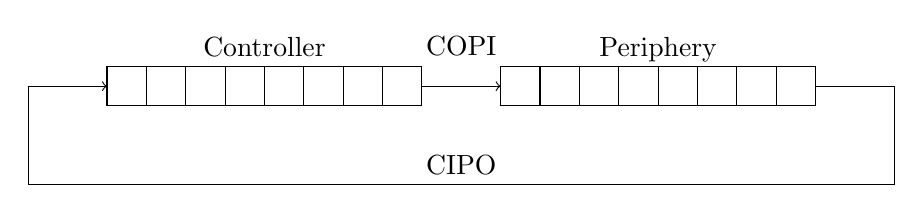
\begin{tikzpicture}
      %% Rectangles.
      \draw[step=0.5cm, black, xshift=0] (0, 0.5) grid (4, 0);
      \draw[step=0.5cm, black, xshift=5cm] (0, 0.5) grid (4, 0);
      %% Arrows.
      \draw[->] (4, 0.25) -- (5, 0.25);
      \draw[->] (9, 0.25)
      -- (10, 0.25)
      -- (10, -1)
      -- (-1, -1)
      -- (-1, 0.25)
      -- (0, 0.25);
      %% Text.
      \node[anchor=north] at (2, 1) {Controller};
      \node[anchor=north] at (7, 1) {Periphery};
      \node[anchor=north] at (4.5, 1) {COPI};
      \node[anchor=south] at (4.5, -1) {CIPO};
    \end{tikzpicture}
    \caption{\figureCaption}
    \label{fig:spi-shift-register}
  \end{figure}
}
